\documentclass[twoside]{book}

% Packages required by doxygen
\usepackage{fixltx2e}
\usepackage{calc}
\usepackage{doxygen}
\usepackage[export]{adjustbox} % also loads graphicx
\usepackage{graphicx}
\usepackage[utf8]{inputenc}
\usepackage{makeidx}
\usepackage{multicol}
\usepackage{multirow}
\PassOptionsToPackage{warn}{textcomp}
\usepackage{textcomp}
\usepackage[nointegrals]{wasysym}
\usepackage[table]{xcolor}

% NLS support packages
\usepackage[french]{babel}

% Font selection
\usepackage[T1]{fontenc}
\usepackage[scaled=.90]{helvet}
\usepackage{courier}
\usepackage{amssymb}
\usepackage{sectsty}
\renewcommand{\familydefault}{\sfdefault}
\allsectionsfont{%
  \fontseries{bc}\selectfont%
  \color{darkgray}%
}
\renewcommand{\DoxyLabelFont}{%
  \fontseries{bc}\selectfont%
  \color{darkgray}%
}
\newcommand{\+}{\discretionary{\mbox{\scriptsize$\hookleftarrow$}}{}{}}

% Page & text layout
\usepackage{geometry}
\geometry{%
  a4paper,%
  top=2.5cm,%
  bottom=2.5cm,%
  left=2.5cm,%
  right=2.5cm%
}
\tolerance=750
\hfuzz=15pt
\hbadness=750
\setlength{\emergencystretch}{15pt}
\setlength{\parindent}{0cm}
\setlength{\parskip}{3ex plus 2ex minus 2ex}
\makeatletter
\renewcommand{\paragraph}{%
  \@startsection{paragraph}{4}{0ex}{-1.0ex}{1.0ex}{%
    \normalfont\normalsize\bfseries\SS@parafont%
  }%
}
\renewcommand{\subparagraph}{%
  \@startsection{subparagraph}{5}{0ex}{-1.0ex}{1.0ex}{%
    \normalfont\normalsize\bfseries\SS@subparafont%
  }%
}
\makeatother

% Headers & footers
\usepackage{fancyhdr}
\pagestyle{fancyplain}
\fancyhead[LE]{\fancyplain{}{\bfseries\thepage}}
\fancyhead[CE]{\fancyplain{}{}}
\fancyhead[RE]{\fancyplain{}{\bfseries\leftmark}}
\fancyhead[LO]{\fancyplain{}{\bfseries\rightmark}}
\fancyhead[CO]{\fancyplain{}{}}
\fancyhead[RO]{\fancyplain{}{\bfseries\thepage}}
\fancyfoot[LE]{\fancyplain{}{}}
\fancyfoot[CE]{\fancyplain{}{}}
\fancyfoot[RE]{\fancyplain{}{\bfseries\scriptsize Généré par Doxygen }}
\fancyfoot[LO]{\fancyplain{}{\bfseries\scriptsize Généré par Doxygen }}
\fancyfoot[CO]{\fancyplain{}{}}
\fancyfoot[RO]{\fancyplain{}{}}
\renewcommand{\footrulewidth}{0.4pt}
\renewcommand{\chaptermark}[1]{%
  \markboth{#1}{}%
}
\renewcommand{\sectionmark}[1]{%
  \markright{\thesection\ #1}%
}

% Indices & bibliography
\usepackage{natbib}
\usepackage[titles]{tocloft}
\setcounter{tocdepth}{3}
\setcounter{secnumdepth}{5}
\makeindex

% Hyperlinks (required, but should be loaded last)
\usepackage{ifpdf}
\ifpdf
  \usepackage[pdftex,pagebackref=true]{hyperref}
\else
  \usepackage[ps2pdf,pagebackref=true]{hyperref}
\fi
\hypersetup{%
  colorlinks=true,%
  linkcolor=blue,%
  citecolor=blue,%
  unicode%
}

% Custom commands
\newcommand{\clearemptydoublepage}{%
  \newpage{\pagestyle{empty}\cleardoublepage}%
}

\usepackage{caption}
\captionsetup{labelsep=space,justification=centering,font={bf},singlelinecheck=off,skip=4pt,position=top}

%===== C O N T E N T S =====

\begin{document}

% Titlepage & ToC
\hypersetup{pageanchor=false,
             bookmarksnumbered=true,
             pdfencoding=unicode
            }
\pagenumbering{alph}
\begin{titlepage}
\vspace*{7cm}
\begin{center}%
{\Large Menu Adaptatif C++ \\[1ex]\large 1.\+1 }\\
\vspace*{1cm}
{\large Généré par Doxygen 1.8.13}\\
\end{center}
\end{titlepage}
\clearemptydoublepage
\pagenumbering{roman}
\tableofcontents
\clearemptydoublepage
\pagenumbering{arabic}
\hypersetup{pageanchor=true}

%--- Begin generated contents ---
\chapter{Index des classes}
\section{Liste des classes}
Liste des classes, structures, unions et interfaces avec une brève description \+:\begin{DoxyCompactList}
\item\contentsline{section}{\hyperlink{classbarre}{barre} \\*The barre class }{\pageref{classbarre}}{}
\item\contentsline{section}{\hyperlink{classbarre_carree}{barre\+Carree} \\*The \hyperlink{classbarre_carree}{barre\+Carree} class }{\pageref{classbarre_carree}}{}
\item\contentsline{section}{\hyperlink{classbarre_hexa_creuse}{barre\+Hexa\+Creuse} \\*The \hyperlink{classbarre_hexa_creuse}{barre\+Hexa\+Creuse} class }{\pageref{classbarre_hexa_creuse}}{}
\item\contentsline{section}{\hyperlink{classbarre_hexagone}{barre\+Hexagone} \\*The \hyperlink{classbarre_hexagone}{barre\+Hexagone} class }{\pageref{classbarre_hexagone}}{}
\item\contentsline{section}{\hyperlink{classbarre_octogone}{barre\+Octogone} \\*The \hyperlink{classbarre_octogone}{barre\+Octogone} class }{\pageref{classbarre_octogone}}{}
\item\contentsline{section}{\hyperlink{classbarre_octogone_creuse}{barre\+Octogone\+Creuse} \\*The \hyperlink{classbarre_octogone_creuse}{barre\+Octogone\+Creuse} class }{\pageref{classbarre_octogone_creuse}}{}
\item\contentsline{section}{\hyperlink{classbarre_rectangle}{barre\+Rectangle} \\*The \hyperlink{classbarre_rectangle}{barre\+Rectangle} class }{\pageref{classbarre_rectangle}}{}
\item\contentsline{section}{\hyperlink{classbarre_ronde}{barre\+Ronde} \\*The \hyperlink{classbarre_ronde}{barre\+Ronde} class }{\pageref{classbarre_ronde}}{}
\item\contentsline{section}{\hyperlink{classbarre_ronde_creuse}{barre\+Ronde\+Creuse} \\*The \hyperlink{classbarre_ronde_creuse}{barre\+Ronde\+Creuse} class }{\pageref{classbarre_ronde_creuse}}{}
\end{DoxyCompactList}

\chapter{Index des fichiers}
\section{Liste des fichiers}
Liste de tous les fichiers avec une brève description \+:\begin{DoxyCompactList}
\item\contentsline{section}{/home/\+U\+S\+E\+R\+S/\+E\+L\+E\+V\+E\+S/\+S\+N\+I\+R2018/gberanger/projet\+Qt/\+S\+N\+I\+R2/\+Apprendre\+\_\+\+Cpp/\+Chapitre\+\_\+2/02\+\_\+\+Menu/\hyperlink{main_8cpp}{main.\+cpp} }{\pageref{main_8cpp}}{}
\item\contentsline{section}{/home/\+U\+S\+E\+R\+S/\+E\+L\+E\+V\+E\+S/\+S\+N\+I\+R2018/gberanger/projet\+Qt/\+S\+N\+I\+R2/\+Apprendre\+\_\+\+Cpp/\+Chapitre\+\_\+2/02\+\_\+\+Menu/\hyperlink{menu_8cpp}{menu.\+cpp} }{\pageref{menu_8cpp}}{}
\item\contentsline{section}{/home/\+U\+S\+E\+R\+S/\+E\+L\+E\+V\+E\+S/\+S\+N\+I\+R2018/gberanger/projet\+Qt/\+S\+N\+I\+R2/\+Apprendre\+\_\+\+Cpp/\+Chapitre\+\_\+2/02\+\_\+\+Menu/\hyperlink{menu_8h}{menu.\+h} }{\pageref{menu_8h}}{}
\end{DoxyCompactList}

\chapter{Documentation des classes}
\hypertarget{class_menu}{}\section{Référence de la classe Menu}
\label{class_menu}\index{Menu@{Menu}}


The \hyperlink{class_menu}{Menu} class.  




{\ttfamily \#include $<$menu.\+h$>$}



Graphe de collaboration de Menu\+:
\nopagebreak
\begin{figure}[H]
\begin{center}
\leavevmode
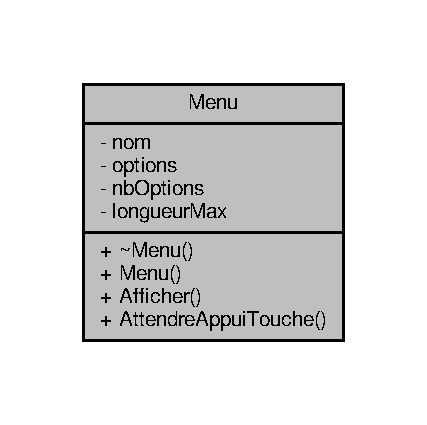
\includegraphics[width=205pt]{class_menu__coll__graph}
\end{center}
\end{figure}
\subsection*{Fonctions membres publiques}
\begin{DoxyCompactItemize}
\item 
\hyperlink{class_menu_a831387f51358cfb88cd018e1777bc980}{$\sim$\+Menu} ()
\item 
\hyperlink{class_menu_a3ec2bde9fc4dfdf5d4e8afcc562fd58f}{Menu} (const string \+\_\+nom)
\begin{DoxyCompactList}\small\item\em \hyperlink{class_menu_a3ec2bde9fc4dfdf5d4e8afcc562fd58f}{Menu\+::\+Menu}. \end{DoxyCompactList}\item 
int \hyperlink{class_menu_a079e0c6a24248a07993b48b310ba65ce}{Afficher} ()
\begin{DoxyCompactList}\small\item\em \hyperlink{class_menu_a079e0c6a24248a07993b48b310ba65ce}{Menu\+::\+Afficher}. \end{DoxyCompactList}\end{DoxyCompactItemize}
\subsection*{Fonctions membres publiques statiques}
\begin{DoxyCompactItemize}
\item 
static void \hyperlink{class_menu_a6ddcaabf2fedb30f5136f3be655d60ce}{Attendre\+Appui\+Touche} ()
\begin{DoxyCompactList}\small\item\em \hyperlink{class_menu_a6ddcaabf2fedb30f5136f3be655d60ce}{Menu\+::\+Attendre\+Appui\+Touche}. \end{DoxyCompactList}\end{DoxyCompactItemize}
\subsection*{Attributs privés}
\begin{DoxyCompactItemize}
\item 
string \hyperlink{class_menu_a99574cb51606811f697854859bc1ccc1}{nom}
\begin{DoxyCompactList}\small\item\em Désigne le nom du fichier. \end{DoxyCompactList}\item 
string $\ast$ \hyperlink{class_menu_aec975cfea9216420d5754ce2e9321390}{options}
\begin{DoxyCompactList}\small\item\em Représente un tableau de chaînes de caractères implémentées sous la forme de string. Ce tableau sera alloué dynamiquement en fonction du nombre de lignes du fichier. \end{DoxyCompactList}\item 
int \hyperlink{class_menu_ad59953635d184fefcddf95015a761187}{nb\+Options}
\begin{DoxyCompactList}\small\item\em Contient le nombre d\textquotesingle{}options du \hyperlink{class_menu}{Menu}. \end{DoxyCompactList}\item 
int \hyperlink{class_menu_a745c540589015b573d8214e1080e2a8e}{longueur\+Max}
\begin{DoxyCompactList}\small\item\em Taille de la plus grande chaîne contenue dans le tableau. \end{DoxyCompactList}\end{DoxyCompactItemize}


\subsection{Description détaillée}
The \hyperlink{class_menu}{Menu} class. 

\begin{DoxyDate}{Date}
13 septembre 2019 
\end{DoxyDate}
\begin{DoxyAuthor}{Auteur}
B\+E\+R\+A\+N\+G\+ER Geoffrey (feat.\+Mathis C) 
\end{DoxyAuthor}


\subsection{Documentation des constructeurs et destructeur}
\mbox{\Hypertarget{class_menu_a831387f51358cfb88cd018e1777bc980}\label{class_menu_a831387f51358cfb88cd018e1777bc980}} 
\index{Menu@{Menu}!````~Menu@{$\sim$\+Menu}}
\index{````~Menu@{$\sim$\+Menu}!Menu@{Menu}}
\subsubsection{\texorpdfstring{$\sim$\+Menu()}{~Menu()}}
{\footnotesize\ttfamily Menu\+::$\sim$\+Menu (\begin{DoxyParamCaption}{ }\end{DoxyParamCaption})}

\mbox{\Hypertarget{class_menu_a3ec2bde9fc4dfdf5d4e8afcc562fd58f}\label{class_menu_a3ec2bde9fc4dfdf5d4e8afcc562fd58f}} 
\index{Menu@{Menu}!Menu@{Menu}}
\index{Menu@{Menu}!Menu@{Menu}}
\subsubsection{\texorpdfstring{Menu()}{Menu()}}
{\footnotesize\ttfamily Menu\+::\+Menu (\begin{DoxyParamCaption}\item[{const string}]{\+\_\+nom }\end{DoxyParamCaption})}



\hyperlink{class_menu_a3ec2bde9fc4dfdf5d4e8afcc562fd58f}{Menu\+::\+Menu}. 


\begin{DoxyParams}{Paramètres}
{\em \+\_\+nom} & \\
\hline
\end{DoxyParams}
Constructeur de la classe \hyperlink{class_menu}{Menu} qui initialise le nom et la longueur\+Max, On verifie si le fichier est ouvert sinon on affiche un msg d\textquotesingle{}erreur, attribution de la valeur longueur\+Max par lecture de toute les lignes du fichier 

\subsection{Documentation des fonctions membres}
\mbox{\Hypertarget{class_menu_a079e0c6a24248a07993b48b310ba65ce}\label{class_menu_a079e0c6a24248a07993b48b310ba65ce}} 
\index{Menu@{Menu}!Afficher@{Afficher}}
\index{Afficher@{Afficher}!Menu@{Menu}}
\subsubsection{\texorpdfstring{Afficher()}{Afficher()}}
{\footnotesize\ttfamily int Menu\+::\+Afficher (\begin{DoxyParamCaption}{ }\end{DoxyParamCaption})}



\hyperlink{class_menu_a079e0c6a24248a07993b48b310ba65ce}{Menu\+::\+Afficher}. 

\begin{DoxyReturn}{Renvoie}

\end{DoxyReturn}
Methode Afficher qui affiche un tableau adaptatif en fonction du nombre d\textquotesingle{}options et de la longueur\+Max de la plus longue option \mbox{\Hypertarget{class_menu_a6ddcaabf2fedb30f5136f3be655d60ce}\label{class_menu_a6ddcaabf2fedb30f5136f3be655d60ce}} 
\index{Menu@{Menu}!Attendre\+Appui\+Touche@{Attendre\+Appui\+Touche}}
\index{Attendre\+Appui\+Touche@{Attendre\+Appui\+Touche}!Menu@{Menu}}
\subsubsection{\texorpdfstring{Attendre\+Appui\+Touche()}{AttendreAppuiTouche()}}
{\footnotesize\ttfamily void Menu\+::\+Attendre\+Appui\+Touche (\begin{DoxyParamCaption}{ }\end{DoxyParamCaption})\hspace{0.3cm}{\ttfamily [static]}}



\hyperlink{class_menu_a6ddcaabf2fedb30f5136f3be655d60ce}{Menu\+::\+Attendre\+Appui\+Touche}. 

Methode Attendre\+Appui\+Touhche qui attends qu\textquotesingle{}on appuie sur une touche pour reafficher le tableau 

\subsection{Documentation des données membres}
\mbox{\Hypertarget{class_menu_a745c540589015b573d8214e1080e2a8e}\label{class_menu_a745c540589015b573d8214e1080e2a8e}} 
\index{Menu@{Menu}!longueur\+Max@{longueur\+Max}}
\index{longueur\+Max@{longueur\+Max}!Menu@{Menu}}
\subsubsection{\texorpdfstring{longueur\+Max}{longueurMax}}
{\footnotesize\ttfamily int Menu\+::longueur\+Max\hspace{0.3cm}{\ttfamily [private]}}



Taille de la plus grande chaîne contenue dans le tableau. 

\mbox{\Hypertarget{class_menu_ad59953635d184fefcddf95015a761187}\label{class_menu_ad59953635d184fefcddf95015a761187}} 
\index{Menu@{Menu}!nb\+Options@{nb\+Options}}
\index{nb\+Options@{nb\+Options}!Menu@{Menu}}
\subsubsection{\texorpdfstring{nb\+Options}{nbOptions}}
{\footnotesize\ttfamily int Menu\+::nb\+Options\hspace{0.3cm}{\ttfamily [private]}}



Contient le nombre d\textquotesingle{}options du \hyperlink{class_menu}{Menu}. 

\mbox{\Hypertarget{class_menu_a99574cb51606811f697854859bc1ccc1}\label{class_menu_a99574cb51606811f697854859bc1ccc1}} 
\index{Menu@{Menu}!nom@{nom}}
\index{nom@{nom}!Menu@{Menu}}
\subsubsection{\texorpdfstring{nom}{nom}}
{\footnotesize\ttfamily string Menu\+::nom\hspace{0.3cm}{\ttfamily [private]}}



Désigne le nom du fichier. 

\mbox{\Hypertarget{class_menu_aec975cfea9216420d5754ce2e9321390}\label{class_menu_aec975cfea9216420d5754ce2e9321390}} 
\index{Menu@{Menu}!options@{options}}
\index{options@{options}!Menu@{Menu}}
\subsubsection{\texorpdfstring{options}{options}}
{\footnotesize\ttfamily string$\ast$ Menu\+::options\hspace{0.3cm}{\ttfamily [private]}}



Représente un tableau de chaînes de caractères implémentées sous la forme de string. Ce tableau sera alloué dynamiquement en fonction du nombre de lignes du fichier. 



La documentation de cette classe a été générée à partir des fichiers suivants \+:\begin{DoxyCompactItemize}
\item 
/home/\+U\+S\+E\+R\+S/\+E\+L\+E\+V\+E\+S/\+S\+N\+I\+R2018/gberanger/projet\+Qt/\+S\+N\+I\+R2/\+Apprendre\+\_\+\+Cpp/\+Chapitre\+\_\+2/02\+\_\+\+Menu/\hyperlink{menu_8h}{menu.\+h}\item 
/home/\+U\+S\+E\+R\+S/\+E\+L\+E\+V\+E\+S/\+S\+N\+I\+R2018/gberanger/projet\+Qt/\+S\+N\+I\+R2/\+Apprendre\+\_\+\+Cpp/\+Chapitre\+\_\+2/02\+\_\+\+Menu/\hyperlink{menu_8cpp}{menu.\+cpp}\end{DoxyCompactItemize}

\chapter{Documentation des fichiers}
\hypertarget{main_8cpp}{}\section{Référence du fichier T\+D\+\_\+\+Barre/main.cpp}
\label{main_8cpp}\index{T\+D\+\_\+\+Barre/main.\+cpp@{T\+D\+\_\+\+Barre/main.\+cpp}}
{\ttfamily \#include $<$iostream$>$}\newline
{\ttfamily \#include \char`\"{}barreoctogonecreuse.\+h\char`\"{}}\newline
Graphe des dépendances par inclusion de main.\+cpp\+:
\nopagebreak
\begin{figure}[H]
\begin{center}
\leavevmode
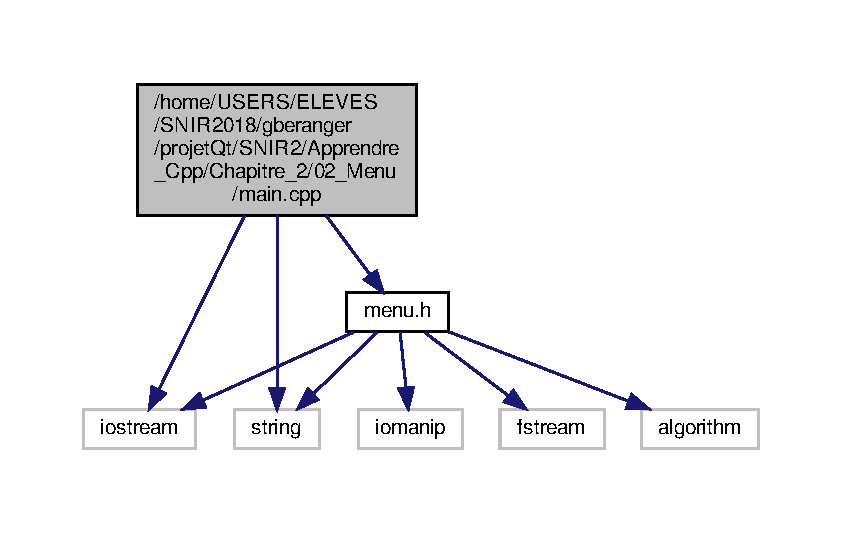
\includegraphics[width=263pt]{main_8cpp__incl}
\end{center}
\end{figure}
\subsection*{Fonctions}
\begin{DoxyCompactItemize}
\item 
int \hyperlink{main_8cpp_ae66f6b31b5ad750f1fe042a706a4e3d4}{main} ()
\begin{DoxyCompactList}\small\item\em main \end{DoxyCompactList}\end{DoxyCompactItemize}


\subsection{Documentation des fonctions}
\mbox{\Hypertarget{main_8cpp_ae66f6b31b5ad750f1fe042a706a4e3d4}\label{main_8cpp_ae66f6b31b5ad750f1fe042a706a4e3d4}} 
\index{main.\+cpp@{main.\+cpp}!main@{main}}
\index{main@{main}!main.\+cpp@{main.\+cpp}}
\subsubsection{\texorpdfstring{main()}{main()}}
{\footnotesize\ttfamily int main (\begin{DoxyParamCaption}{ }\end{DoxyParamCaption})}



main 

\begin{DoxyVersion}{Version}
1.\+0 
\end{DoxyVersion}
\begin{DoxyDate}{Date}
20/09/2019
\end{DoxyDate}
Programme Principal qui créer une barre en initialisant ses paramètres, Puis affiche sa Section et sa Masse \begin{DoxyReturn}{Renvoie}

\end{DoxyReturn}
Création d\textquotesingle{}un objet Barre\+Octogone\+Creuse

Affichage de la section de cette barre

Affichage de la Masse de cette Barre 
\hypertarget{menu_8cpp}{}\section{Référence du fichier /home/\+U\+S\+E\+R\+S/\+E\+L\+E\+V\+E\+S/\+S\+N\+I\+R2018/gberanger/projet\+Qt/\+S\+N\+I\+R2/\+Apprendre\+\_\+\+Cpp/\+Chapitre\+\_\+2/02\+\_\+\+Menu/menu.cpp}
\label{menu_8cpp}\index{/home/\+U\+S\+E\+R\+S/\+E\+L\+E\+V\+E\+S/\+S\+N\+I\+R2018/gberanger/projet\+Qt/\+S\+N\+I\+R2/\+Apprendre\+\_\+\+Cpp/\+Chapitre\+\_\+2/02\+\_\+\+Menu/menu.\+cpp@{/home/\+U\+S\+E\+R\+S/\+E\+L\+E\+V\+E\+S/\+S\+N\+I\+R2018/gberanger/projet\+Qt/\+S\+N\+I\+R2/\+Apprendre\+\_\+\+Cpp/\+Chapitre\+\_\+2/02\+\_\+\+Menu/menu.\+cpp}}
{\ttfamily \#include \char`\"{}menu.\+h\char`\"{}}\newline
Graphe des dépendances par inclusion de menu.\+cpp\+:\nopagebreak
\begin{figure}[H]
\begin{center}
\leavevmode
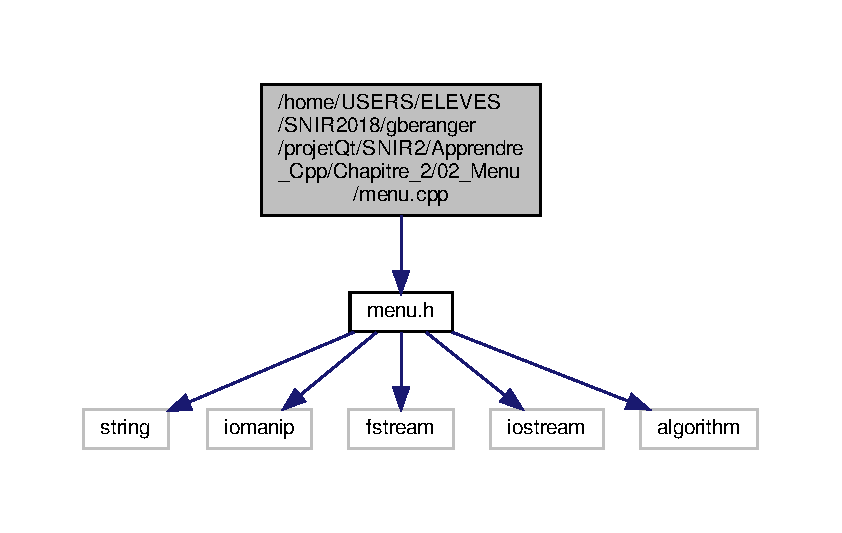
\includegraphics[width=350pt]{menu_8cpp__incl}
\end{center}
\end{figure}

\hypertarget{menu_8h}{}\section{Référence du fichier /home/\+U\+S\+E\+R\+S/\+E\+L\+E\+V\+E\+S/\+S\+N\+I\+R2018/gberanger/projet\+Qt/\+S\+N\+I\+R2/\+Apprendre\+\_\+\+Cpp/\+Chapitre\+\_\+2/02\+\_\+\+Menu/menu.h}
\label{menu_8h}\index{/home/\+U\+S\+E\+R\+S/\+E\+L\+E\+V\+E\+S/\+S\+N\+I\+R2018/gberanger/projet\+Qt/\+S\+N\+I\+R2/\+Apprendre\+\_\+\+Cpp/\+Chapitre\+\_\+2/02\+\_\+\+Menu/menu.\+h@{/home/\+U\+S\+E\+R\+S/\+E\+L\+E\+V\+E\+S/\+S\+N\+I\+R2018/gberanger/projet\+Qt/\+S\+N\+I\+R2/\+Apprendre\+\_\+\+Cpp/\+Chapitre\+\_\+2/02\+\_\+\+Menu/menu.\+h}}
{\ttfamily \#include $<$string$>$}\newline
{\ttfamily \#include $<$iomanip$>$}\newline
{\ttfamily \#include $<$fstream$>$}\newline
{\ttfamily \#include $<$iostream$>$}\newline
{\ttfamily \#include $<$algorithm$>$}\newline
Graphe des dépendances par inclusion de menu.\+h\+:\nopagebreak
\begin{figure}[H]
\begin{center}
\leavevmode
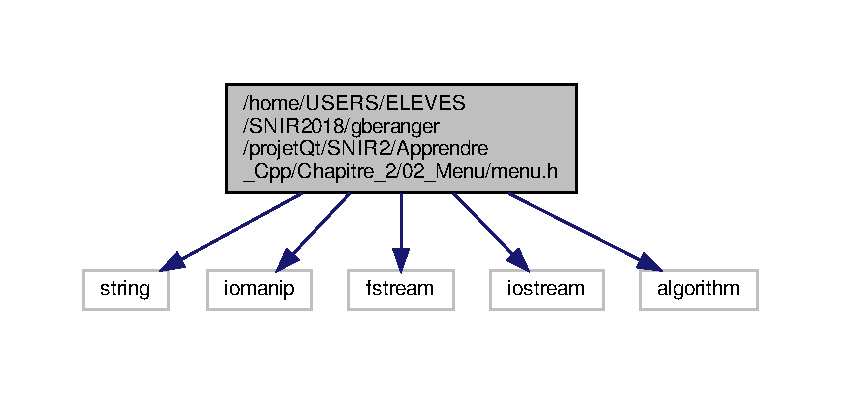
\includegraphics[width=350pt]{menu_8h__incl}
\end{center}
\end{figure}
Ce graphe montre quels fichiers incluent directement ou indirectement ce fichier \+:\nopagebreak
\begin{figure}[H]
\begin{center}
\leavevmode
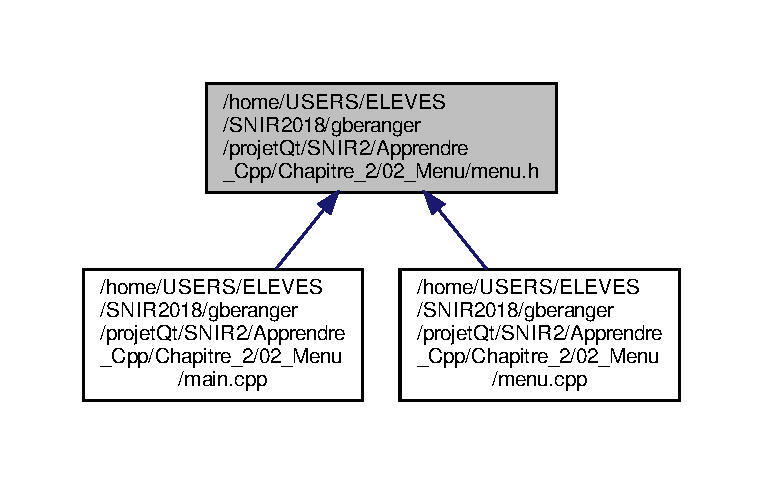
\includegraphics[width=350pt]{menu_8h__dep__incl}
\end{center}
\end{figure}
\subsection*{Classes}
\begin{DoxyCompactItemize}
\item 
class \hyperlink{class_menu}{Menu}
\begin{DoxyCompactList}\small\item\em The \hyperlink{class_menu}{Menu} class. \end{DoxyCompactList}\end{DoxyCompactItemize}

%--- End generated contents ---

% Index
\backmatter
\newpage
\phantomsection
\clearemptydoublepage
\addcontentsline{toc}{chapter}{Index}
\printindex

\end{document}
